\usetikzlibrary{arrows.meta}

\begin{frame}{connected sockets}
    \begin{itemize}
    \item sockets can represent a connection
    \end{itemize}
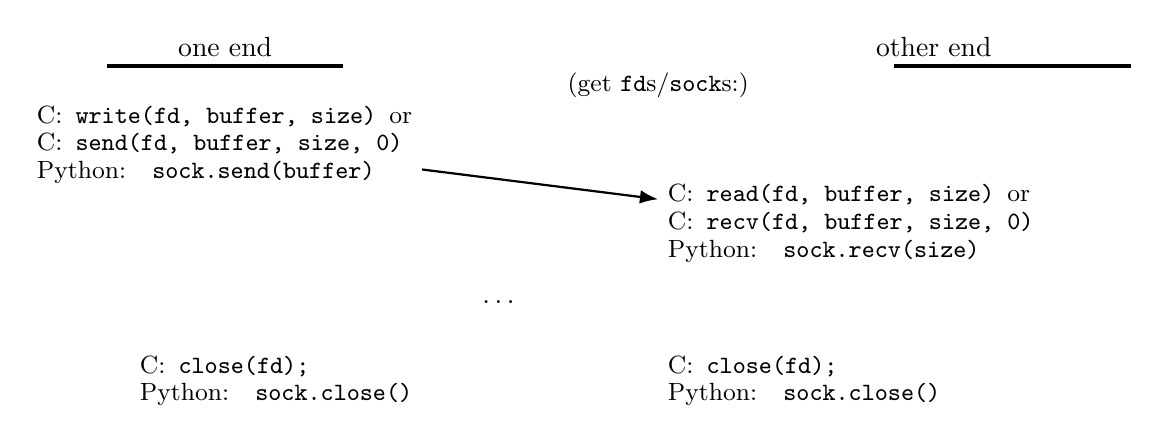
\begin{tikzpicture}
\tikzset{>=Latex}
\node[anchor=south] at (1.5, 0) {one end};
\draw[ultra thick] (0, 0) -- ++(3, 0);
\draw[ultra thick] (10, 0) -- ++(3, 0);
\node[anchor=south] at (10.5, 0) {other end};
\node[font=\small] at (7, -.25) {(get \texttt{fd}s/\texttt{sock}s:)};
\tikzset{
    function/.style={font=\fontsize{9}{10}\tt\selectfont,align=left},
}
\node[function,anchor=east] (write 1) at (4, -1) {
{\normalfont C:} write(fd, buffer, size) \textit{\normalfont or} \\
{\normalfont C:} send(fd, buffer, size, 0) \\
{\normalfont Python:} sock.send(buffer) 
};
\node[function,anchor=west] (read 1) at (7, -2) {
{\normalfont C:} read(fd, buffer, size) \textit{\normalfont or} \\
{\normalfont C:} recv(fd, buffer, size, 0) \\
{\normalfont Python:} sock.recv(size) 
};
\draw[thick,->] (write 1) -- (read 1);
\node at (5, -3) {\ldots};
\node[function,anchor=east] at (4, -4) {
    {\normalfont C:} close(fd); \\
    {\normalfont Python:} sock.close()
};
\node[function,anchor=west] at (7, -4) {
    {\normalfont C:} close(fd); \\
    {\normalfont Python:} sock.close()
};
\end{tikzpicture}
\end{frame}

